\documentclass[parskip=full,11pt,twoside]{scrartcl}
\usepackage[utf8]{inputenc}

\title{GO-App}
\author{Lukas Dippon, Jens Kienle, Matthias Noll, Fabian Röpke, Tim Schmidt, Simon Vögele}

% section numbers in margins:
\renewcommand\sectionlinesformat[4]{\makebox[0pt][r]{#3}#4}

% header & footer
\usepackage{scrlayer-scrpage}
\lofoot{\today}
\refoot{\today}
\pagestyle{scrheadings}

%\usepackage[sfdefault,light]{roboto}
\usepackage[T1]{fontenc}
\usepackage[german]{babel}
\usepackage[yyyymmdd]{datetime} % must be after babel
\renewcommand{\dateseparator}{-} % ISO8601 date format
\usepackage{hyperref}
\usepackage[nameinlink]{cleveref}
\crefname{figure}{Abb}{Abb}
\usepackage[section]{placeins}
\usepackage{xcolor}
\usepackage{graphicx}
\hypersetup{
	pdftitle={Pflichtenheft},
	bookmarks=true,
}
\usepackage{csquotes}

\usepackage{amsmath} % for $\text{}$
\newcommand\urlpart[2]{$\underbrace{\text{\texttt{#1}}}{\text{#2}}$}

\usepackage{pflichtenheft}

\begin{document}
\maketitle

\section{Einleitung}

Studenten und Mitarbeiter des KIT treffen sich gerne zum gemeinsamen Essen oder Lernen.
Dazu ist an einem bestimmten Tag immer notwendig zu wissen, ob bereits ein Treffen vereinbart wurde.
Am Treffpunkt angekommen, möchte man wissen, an welchem Ort sich die Gruppe befindet, um nicht lange suchen zu müssen.
Unsere App soll es angemeldeten Benutzern ermöglichen, sich in Gruppen zu organisieren.
In den Gruppen kann der Zeit- und Treffpunkt bestimmt werden.
Nach der Festlegung des Treffens soll die App die GPS-Standorte der Mitglieder temporär und anonym anzeigen, um das Treffen zu vereinfachen.

\pagebreak
\section{Kriterien}
% Diese Section sollte kurz und knapp "für Manager" sein
% und auf eine Seite passen.

\subsection{Muss}

\criterium{Vereinfachte Treffpunkte}{crt:easy}
Durch das Freigeben von Positionsdaten können andere Nutzer den
Standort bestimmen.

\criterium{Datenschutz}{crt:safe}
Die Positionsdaten werden nur mit Bestätigung
des Nutzers gesendet und serverseitig nicht längerfristig gespeichert.

\criterium{Gruppen}{crt:groups}
Mehrere Nutzer können sich in Gruppen zusammenschließen. In diesen
können sie Positionsdaten austauschen und Treffpunkte festlegen.
Ein Nutzer kann in beliebig vielen Gruppen Mitglied sein.

\criterium{1 zu 1 Verbindung}{crt:1to1}
Die Position kann auf Wunsch auch mit nur mit einem anderen Nutzer geteilt werden

\criterium{Account}{crt:acc}
Ein persönlicher Account ermöglicht es allen Nutzern,
Gruppenzugehörigkeiten und Datenschutzoptionen zu speichern.

\subsection{Kann}

\criteriumOptional{Abstimmungen}{crt:vote}
Innerhalb von Gruppen können die Nutzer z.B. über nächste Treffpunkte abstimmen

\criteriumOptional{Detailliertere Innenraumkarten}{crt:indoor}
Innenräume mit hoher Nutzerdichte bekommen detaillierte Innenraumkarten.

\criteriumOptional{Seite mit Betreiberinfo}{crt:about}
Der Dienst bietet eine Seite \enquote{Über Uns},
mit Informationen zum Betreiber.

\subsection{Abgrenzung}

\criteriumNot{Keine Wahl Kurz-URL}{crt:no-choice}
Ein Nutzer hat keine Möglichkeit die Auswahl einer Kurz-URL zu beeinflussen.

\pagebreak
%%%%%%%%%%%%%%
\section{Produkteinsatz}

Das Produkt soll mit minimalen Administrationskenntnissen zu betreiben sein.

Besucher des Diensts sollen diesen ohne Schulung oder andere Information benutzen können.

\section{Produktumgebung}

Das Programm soll als Servlet in einem Apache Tomcat betrieben werden.

Es stehen mindestens 2 AMD64 Kerne mit insgesamt 2GB shared RAM zur Verfügung.

%%%%%%%%%%%
\section{Funktionale Anforderungen}

\functionality{Homepage der App unterteilt in Tabs für die unterschiedlichen Funktionen}{fnc:ui}\label{FA1}
- Liste aller Gruppen, in denen man Mitglied ist (\ref{FA4})
- Liste aller Events, an welchen man teilnimmt (\ref{FA11})
- Einstellungen(\ref{FA3})

\functionality{Login in einen appspezifischen Account}{fnc:login}\label{FA2}
\fullfills{crt:acc}
Der Benutzer muss sich vor der Nutzung der App einen Account erstellen und sich mit diesem einloggen

\functionality{Verwaltung von Einstellungen und Account- oder appbezogene Daten}{fnc:options}\label{FA3}
\fullfills{crt:acc}
ERROR 404 "Beschreibung" not found

\functionality{Gründen von Gruppen}{fnc:groupfounding}\label{FA4}
\fullfills{crt:groups}
Über einen Reiter im Hauptmenü können Gruppen erstellt werden. Ihre Funktionen werden in \ref{FA5} bis \ref{FA10} beschrieben.

\functionality{Gruppenmenü}{fnc:groupmenu}\label{FA5}
\fullfills{crt:groups}
Jede Gruppe besitzt ein eigenes Menü über welches ihre Funktionen angesteuert werden können:
- Umgebungskarte (\ref{FA8})
- Anfrage von GPS-Standorten (\ref{FA9})
- Erstellen eines Events (\ref{FA11} und \ref{FA12})
- Einladen von Mitgliedern (\ref{FA6})
- Liste aller Mitglieder (\ref{FA7})

\functionality{Einladen von Mitgliedern}{fnc:invitations}\label{FA6}
\fullfills{crt:groups}
Es können Einladungen an Nutzer versandt. Diese können von den eingeladenen Nutzern akzeptiert oder abgelehnt werden.

\functionality{Liste der Gruppenmitglieder}{fnc:memberlist}\label{FA7}
\fullfills{crt:groups}
Es werden alle Mitglieder aufgelistet. Durch das Anklicken eines Mitgliedes kann wahlweise das zugehörige Profil besucht oder das Mitglied aus der Gruppe entfernt werden.

\functionality{Umgebungskarte}{fnc:map}\label{FA8}
\fullfills{crt:groups}
\fullfills{crt:easy}
Jede Gruppe verfügt über eine Umgebungskarte mit eigenem Standort.

\functionality{Anfrage von GPS-Standorten}{fnc:locationrequest}\label{FA9}
\fullfills{crt:groups}
\fullfills{crt:easy}
Erstellen einer GPS-Anfrage, bei der alle Gruppenmitglieder über ein Pop-Up gebeten werden ihren Standort für einen fest definierten Zeitraum freizugeben

\functionality{Anzeigen von anonymen GPS-Standorten}{fnc:locations}\label{FA10}
\fullfills{crt:easy}
\fullfills{crt:safe}
Alle GPS-Standorte der Grupenmitglieder, die aktuell freigestellt sind, werden erfasst und als Gruppierungen auf der in \ref{FA8} beschriebenen Gruppenkarte markiert. Diese Gruppierungen bestehen aus geographisch nah beieinanderliegenden Gruppenmitgliedern. Einzelpersonen werden dabei als blaue Dreiecke, mit Spitze nach unten, dargestellt. Das Symbol für Gruppierungen dagegen besteht aus drei solchen Dreiecken, die sich teilweise überlappen. Das Gruppierungssymbol wird außerdem durch eine kleine Zahl begleitet, die die Größe der Gruppierung beschreibt.

\functionality{Events}{fnc:events}\label{FA11}
Gruppenmitglieder können ein Event, bestehend aus Ort und einen Zeit, definieren. Das Event wird mit Uhrzeit in der Eventliste(\ref{FA15}) aufgelistet und als roter Punkt mit Uhrzeit auf der Karte (\ref{FA8}) markiert. Die Mitglieder werden eine kurze Zeit vor dem Event automatisch von der App über ein Pop-Up gebeten, ihren Standort temporär freizugeben.

\functionality{Abstimmungen}{fnc:vote}\label{FA12}
\fullfills{crt:vote}
Das Event(\ref{FA11}) lässt sich durch eine Abstimmung vereinbaren. Diese ist zeitlich begrenzt durch eine vom Ersteller festgelegte Zeit. Hierbei können inerhalb der Zeitgrenze beliebig oft von den Gruppenmitgliedern Orte und Zeitpunkte hinzugefügt werden, die eigene Stimme verändert, oder die Zeitgrenze verlängert werden.

\functionality{Anzeigen von Treffpunkten}{fnc:meetingpoints}\label{FA13}
\fullfills{crt:vote}
\fullfills{crt:easy}
Während einer Abstimmung werden alle möglichen Orte auf der Karte (\ref{FA8}) als orangene Punkte angezeigt. Durch das Anklicken des Ortes in der Abstimmung lassen sich die Markierungen auf der Karte erreichen. Nach Vollendung der Abstimmung wird der Ort mit den meisten Stimmen als finaler Treffpunkt festgelegt, während alle anderen Orte von der Karte gelöscht werden.

\functionality{Standortteilung für einzelne Personen}{fnc:1to1}\label{FA14}
\fullfills{crt:1to1}
\fullfills{crt:easy}
Es soll auch für Einzelpersonen möglich sein ihren Standort zu teilen. Dies soll intern als Zweiergruppe implementiert sein, aber in der App als extra Reiter schnell und ohne den Umweg über die Gruppengründung möglich sein.

\functionality{Eventliste}{fnc:eventlist}\label{FA15}
Alle vereinbarten Treffen werden nach Zeitpunkt sortiert angezeigt. Das Auswählen eines Treffens zeigt die aktuelle Umgebungskarte(\ref{FA8}) der entsprechenden Gruppe an.

%%%%%%%%%%%
\section{Nicht-Funktionale Anforderungen}

\nonFunctionality{Modernes Design}{nfc:design}

Das Design soll modern und seriös wirken.

\nonFunctionality{Persistenz}{nfc:persistence}

Sollten in Zukunft Erweiterungen oder Updates notwendig werden,
müssen die Daten (Kurz-URLs, E-Mailaddressen) erhalten bleiben.

\nonFunctionality{Erweiterbarkeit}{nfc:extensibility}

Das Produkt muss dahingehend erweiterbar sein,
das die Liste der E-Mail-URL Abbildung von authentifizierten Nutzern
abgerufen werden kann.
Wie das genau implementiert wird, ist nicht Teil dieses Projekts.

%%%%%%%%%%%
\section{Tests}

\test{Kurz-URL Erstellen}{tst:create}
\tests{fnc:login}

\teststep{Besucher \enquote{Zoe Washburne} hat einen Browser geöffnet.}
{Zoe navigiert auf die Homepage \texttt{http://atu.rl/}.}
{Die Homepage wird angezeigt wie in \cref{fig:homepage}.}

\teststep{Zoe hat einen Facebook-Account.}%
{Zoe drückt den \enquote{Login via Facebook} Knopf.}%
{Zoe wird eingeloggt und auf die Erstellseite wie in \cref{fig:form} weitergeleitet.}

\teststep{}
{Zoe befüllt das Feld \enquote{URL} mit \texttt{sehrlangedomain.com/undganzlangeURL.html} und drückt auf \enquote{Kurz-URL erstellen}.}%
{Ihr wird eine Kurz-URL angezeigt wie z.B.\ \texttt{atu.rl/abc}
 wie in \cref{fig:generated}.
 Statt \enquote{abc}, dürfen beliebige andere Buchstaben und Zahl angezeigt werden, allerdings exakt drei.}

\teststep{}
{Zoe navigiert auf die eben generierte Kurz-URL, z.B.\ \texttt{http://atu.rl/abc}.}
{Sie wird zu \texttt{sehrlangedomain.com/undganzlang  eURL.html} weitergeleitet.}

\test{Betreiberinfos lesen}{tst:tmg}
\tests{fnc:impressum-link}
\tests{fnc:datenschutz-link}

\teststep{Besucher \enquote{Jayne Cobb} ist auf der Homepage}
{Er folgt dem Link mit dem Text \enquote{Datenschutz}}
{Ein Text mit allen Datenschutzinformationen wird ihm angezeigt.}

\teststep{}
{Jayne folgt dem Link mit dem Text \enquote{Impressum}}
{Ein Text mit Informationen des Betreibers wird ihm angezeigt.}

%%%%%%%%%%%%%
\pagebreak
\appendix

\section{Seitenentwürfe}

% made via https://gomockingbird.com/projects/mnf0cwf/4gXVnC

\begin{figure}[hb]
	\fbox{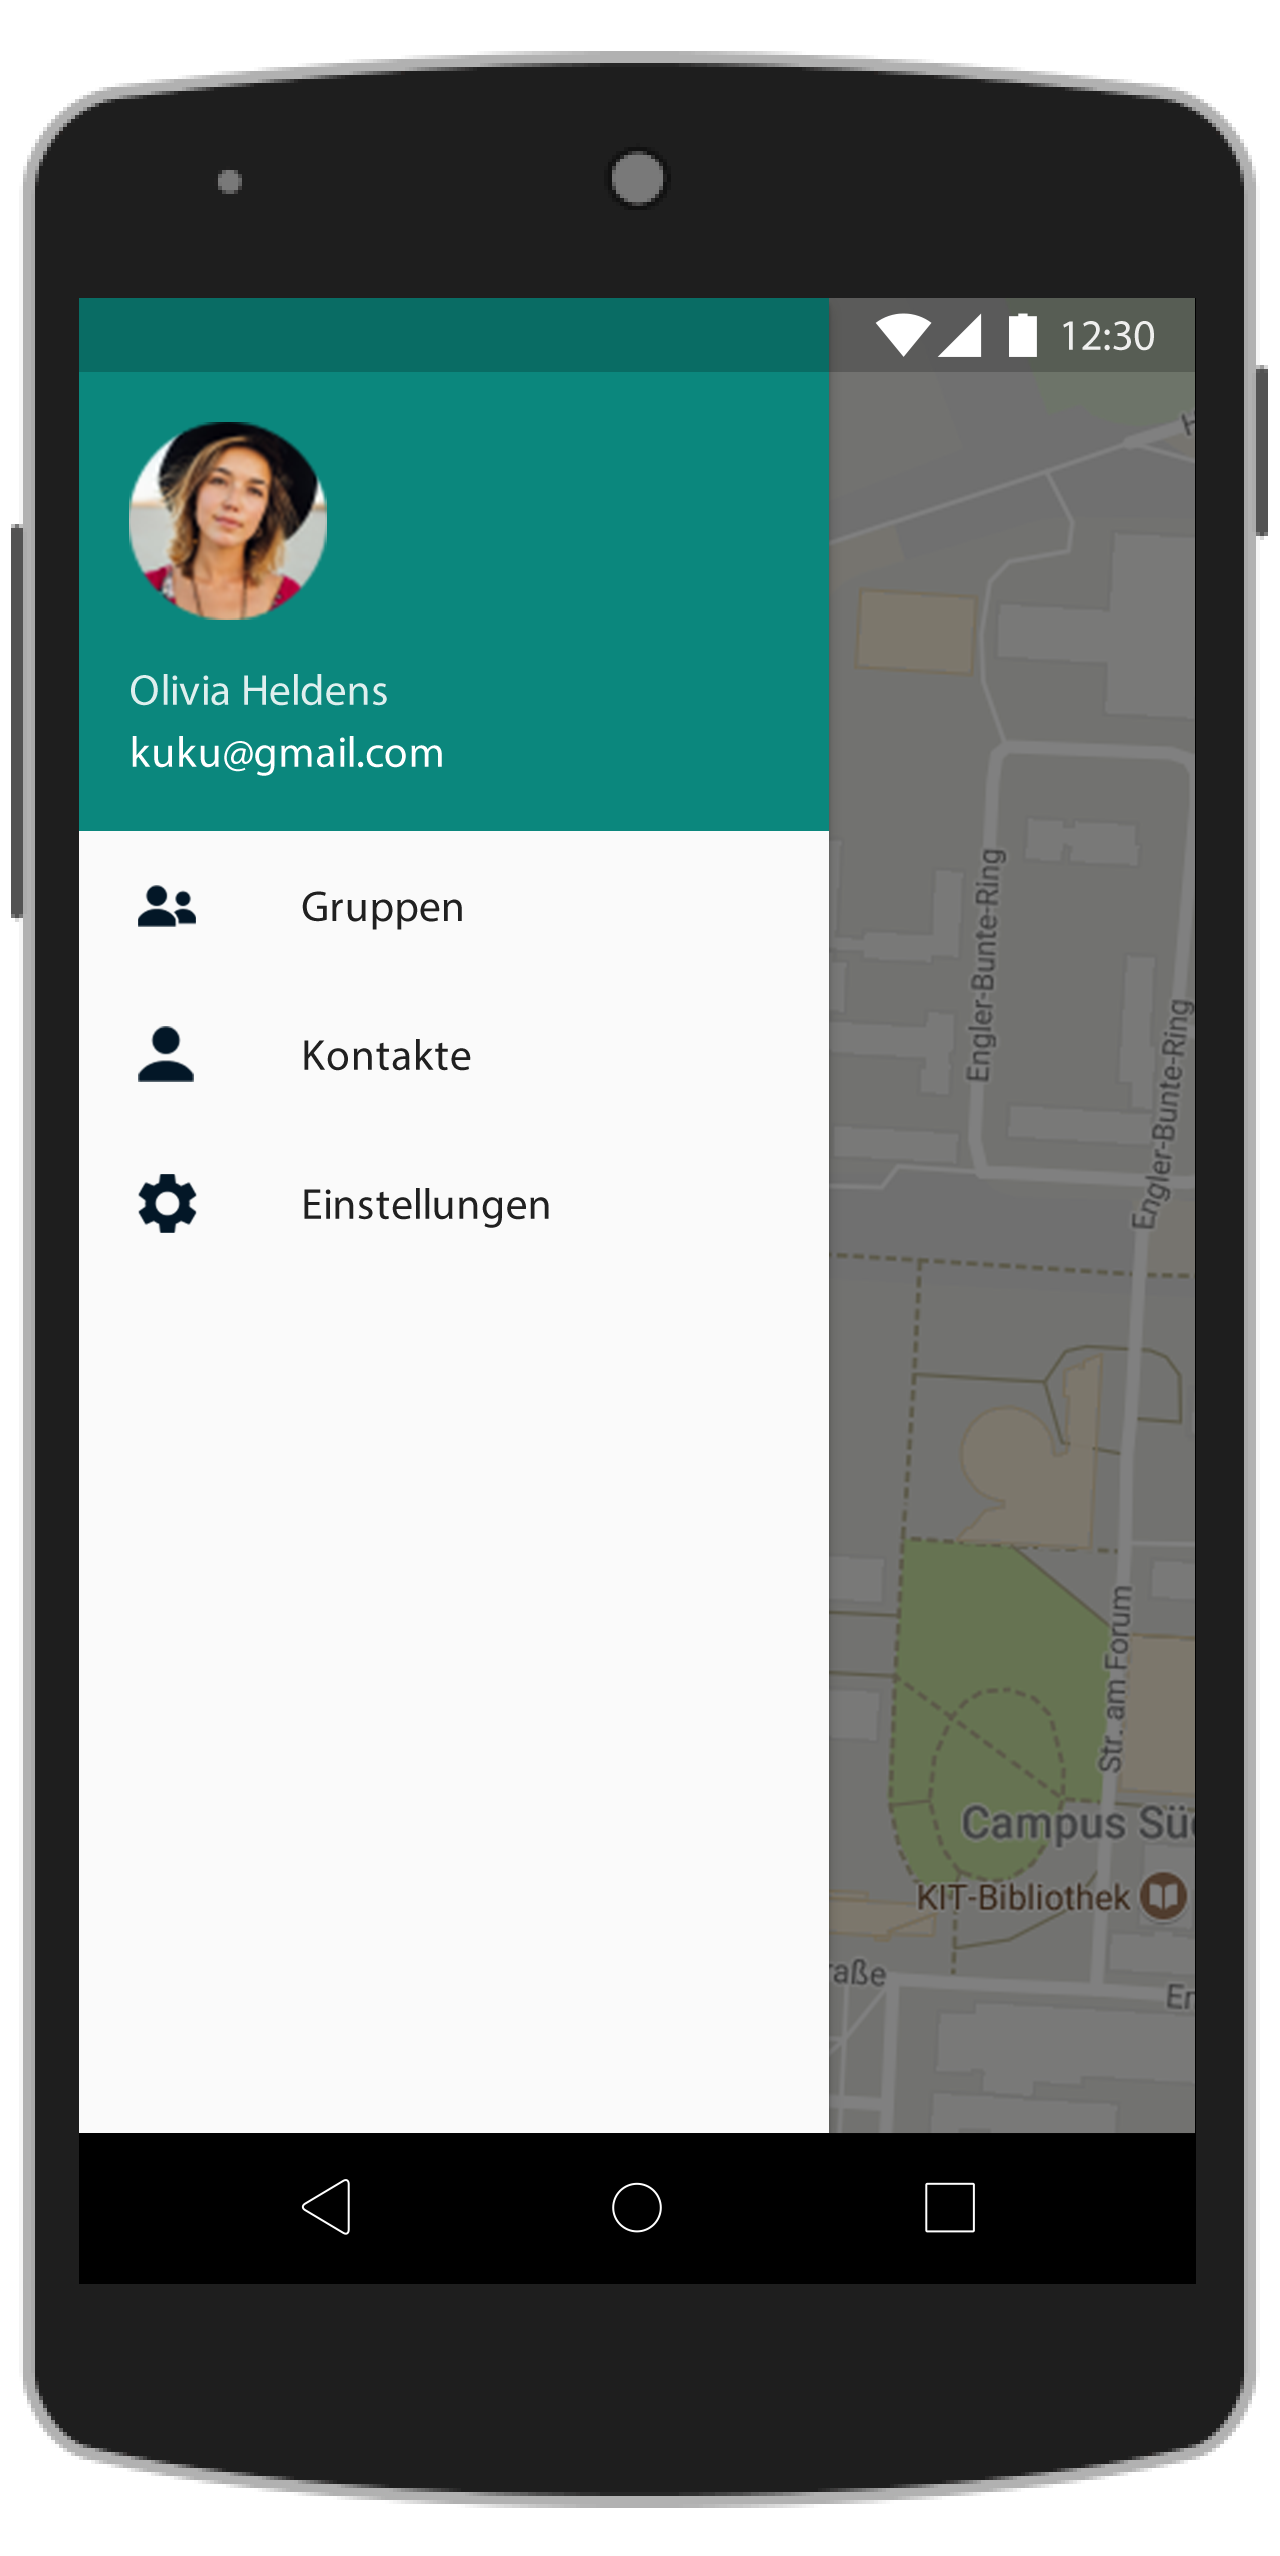
\includegraphics[height=80mm]{screenshots/menu.png}}
	\caption{\label{fig:menu}
		Menü mit der Möglichkeit auf Gruppen, Kontakte und Einstellungen zuzugreifen.
		 \testlink{tst:create}.
	}
\end{figure}

\begin{figure}[hb]
		\fbox{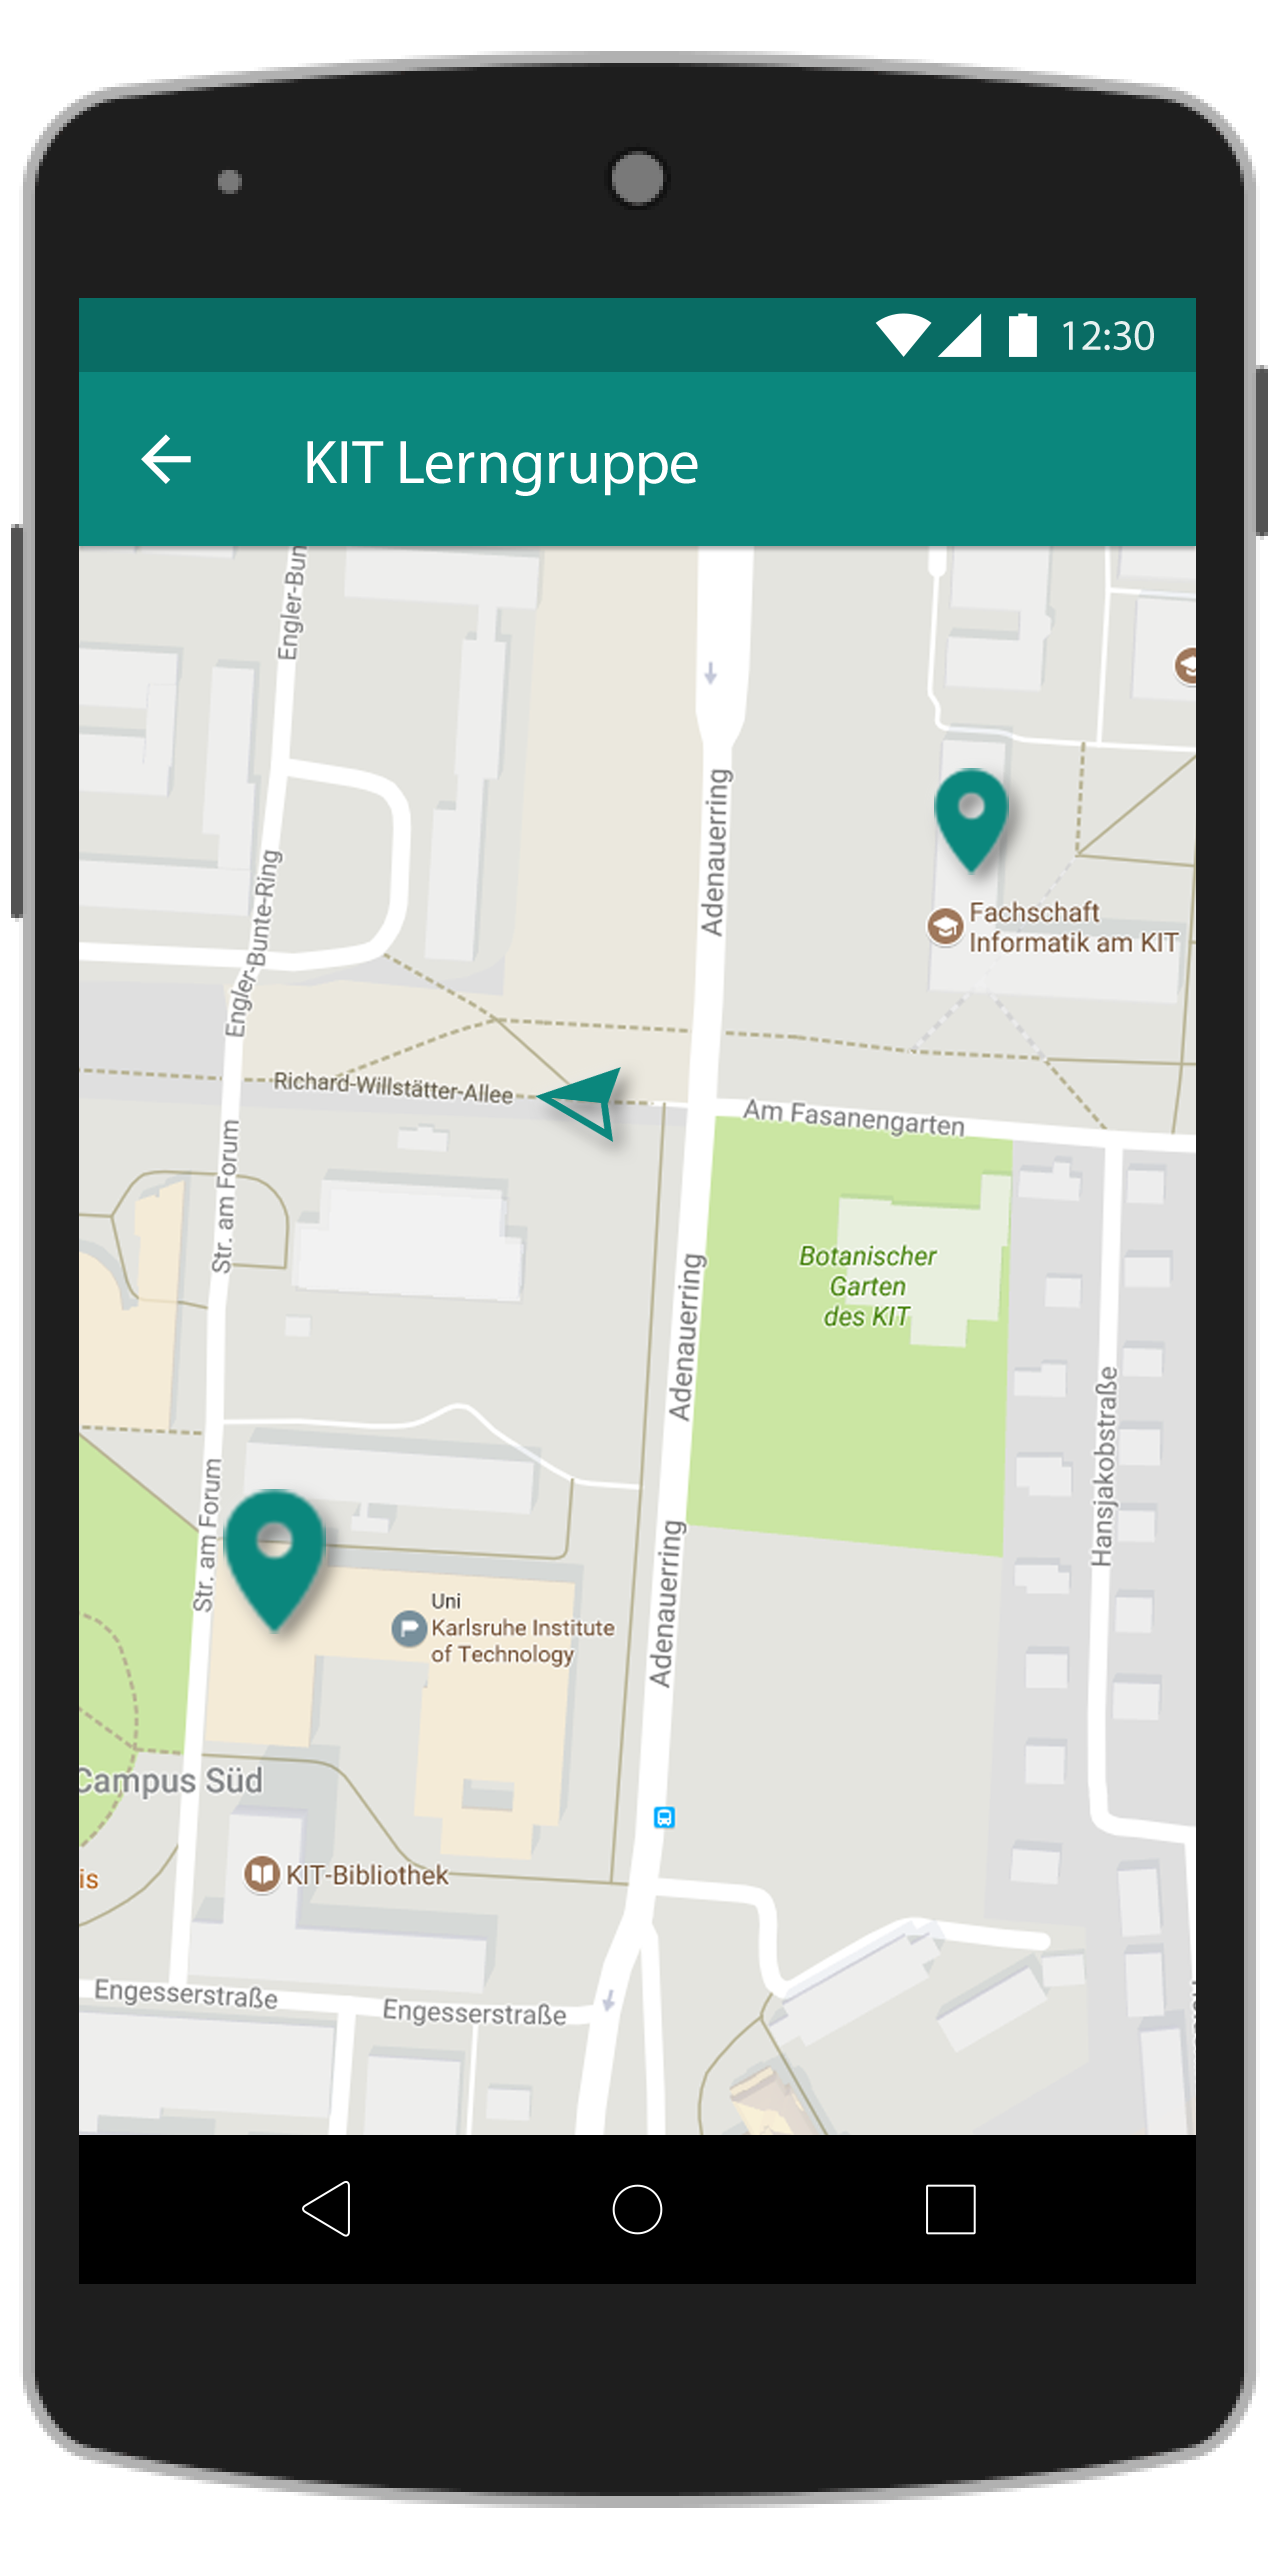
\includegraphics[height=80mm]{screenshots/karte.png}}
		\caption{\label{fig:map}
			Auf der Karte kann die Position der anderen Gruppenmitglieder eingesehen werden.
			Orte mit mehreren Mitgliedern erscheinen größer. 
			\testlink{tst:create}.
		}
\end{figure}

\begin{figure}[hb]
		\fbox{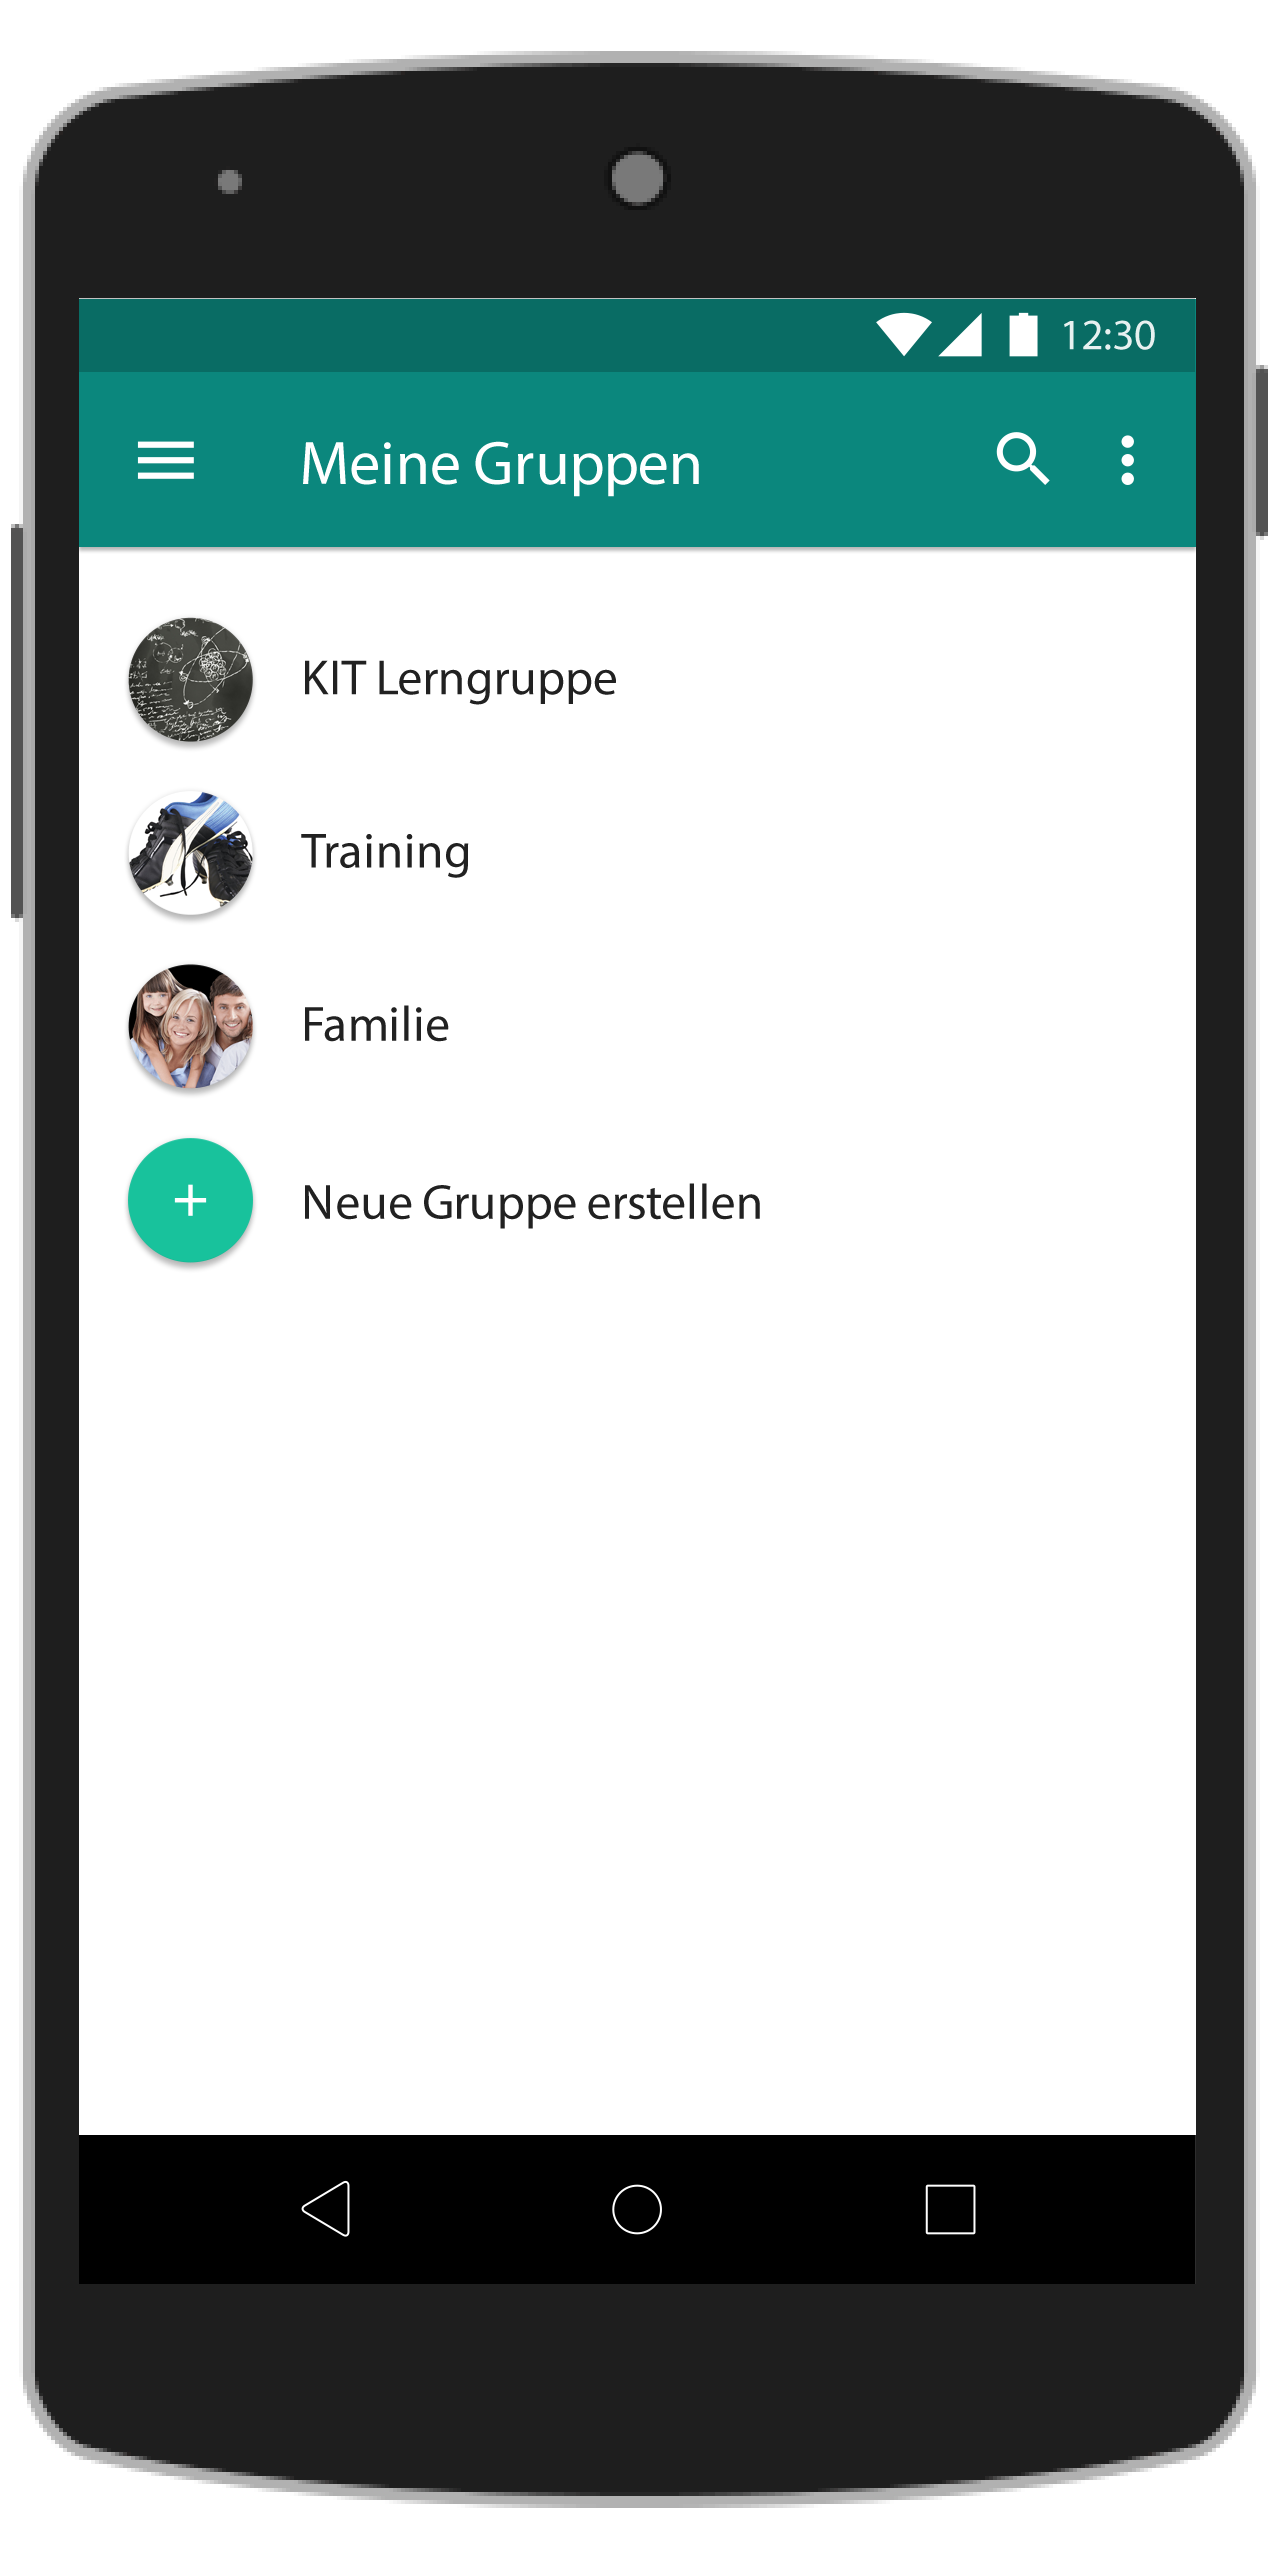
\includegraphics[height=80mm]{screenshots/gruppen.png}}
		\caption{\label{fig:groups}
			Hier können Gruppen verwaltet und angesehen, sowie neue hinzugefügt werden.
			\testlink{tst:create}.
		}
\end{figure}

\section{Glossar}

\textbf{Besucher}:
Eine Person, welche den Dienst nutzt.
Kann eingeloggt sein oder nicht.

\textbf{Dienst}:
Die Software im laufenden Betrieb. Software as a Service.

\textbf{Homepage}:
Seite, die beim Besuchen der Betreiberdomain \emph{ohne Pfad} angezeigt wird. Auch \enquote{Startseite}.

\textbf{Nutzer}:
Ein eingeloggter Besucher.

\end{document}
